% !TeX root = ./main.tex

\section*{Shapovalov form}

Geordie suggested computing the Gram matrix of the Shapovalov form in the basis of MV cycles for the spherical Schubert varieties. 

Let us try.

\subsection*{Useful property of the MV basis}

\begin{definition}
    $B$ is a \new{perfect} basis of $\CC[U]$ if 
    \begin{itemize}
        \item $1_U\in B$
        \item each $b\in B$ is \textit{homogeneous} of degree $\wt(b)$ wrt the $Q_+$ grading on $\CC[U]$
        \item for each $i\in I$ and for each $b\in B$
        \begin{equation}
            e_i \cdot b - \varepsilon_i(b) \tilde e_i (b) \in \Sp(\{b'\in B : \varepsilon_i(b') < \varepsilon_i(b) - 1\})
        \end{equation}
    \end{itemize}
\end{definition}

\begin{example}[The example that they like to give] % the only example they know :S 
    Let $G=\SL_3$ and identify $\CC[U] = \CC[x,y,z]$ by coordinatizing elements of $U\le G$ as 
    \[
    (x,y,z) \in \AA^3 \mapsto \begin{bmatrix}
        1 & x & z \\
          & 1 & y \\
          &   & 1 
    \end{bmatrix} \in U    
    \]
    In this case there is just one perfect basis \cite{XYZ} of $\CC[U]$ and it is
    \begin{equation}
        B = \{
            x^a z^b (xy-z)^c : a,b,c \in \ZZ_{\ge 0}    
        \} \cup \{
            y^a z^b (xy-z)^c : a,b,c \in \ZZ_{\ge 0}  
        \}
    \end{equation}
    % 
    Note that $xy-z$ is homogeneous as $\wt(x) + \wt(y) = \alpha_1 + \alpha_2 = \wt (z)$. 
    % 
    The Lie algebra $\cU\n$ acts on $B$ via 
    \begin{equation}
        e_1 = \partial_x \qquad e_2 = \partial_y + x \partial_z
    \end{equation}
    % 
    Let's check that 
    \[
        \partial_xb = \varepsilon_1(b) \tilde e_1 (b) + \sum_{\varepsilon_1(b') < \varepsilon_1(b) - 1} c(b') b'
    \]
    and 
    \[
        \partial_y + x \partial_zb = \varepsilon_2(b) \tilde e_2(b) + \sum_{\varepsilon_2(b') < \varepsilon_2(b) - 1} c(b') b'  
    \]
    in some examples. 

    First, recall that a Lusztig datum $n_\bullet^{\uvi} = (n_1,n_2,\dots,n_\ell)$ associated to a partition of $\nu\in Q_+$ defines a minor as follows. 
    % 
    \[
        \Delta(n_\bullet) = \Delta_{12..n-1,w(12..n-1)} \qquad w=
    \]
    % 

    Fix $\uvi = (1,2,1)$. 


    {\bf The case $b=z = \Delta_{1,3}$.} This element has $n_\bullet = (1,0,1)$ since $3 = s_1 s_2 (1)$. In terms of tableaux
    \[
        \tau(b) = \young(13,2) \in B(\omega_1 + \omega_2)
    \]
    and 
    \[
        \varepsilon_1(\tau) \tilde e_1 (\tau) = 0  \qquad \varepsilon_2(\tau) \tilde e_2 (\tau) = \young(12,2)    
    \]
    Directly, 
    \[
        \partial_x z = 0 \qquad (\partial_y + x \partial_z)z = x    
    \]
    Indeed $n_\bullet(\young(12,2)) = (1,0,0)$ agrees with the fact that $x = \Delta_{1,2}$ as $s_1(1) = 2$. 
    
    {\bf The case $b = xy-z = \Delta_{12,23}$.} This element has $n_\bullet = (0,1,0)$ since $23 = s_2s_1(12)$. In terms of tableaux
    \[
        \tau(b) = \young(12,3) \in B(\omega_1 + \omega_2)
    \]
    and 
    \[\varepsilon_1(\tau) \tilde e_1 (\tau) = \young(11,3)  \qquad \varepsilon_2(\tau) \tilde e_2 (\tau) = 0 \]
    Directly, 
    \[
        \partial_x (xy-z) = y \qquad (\partial_y + x \partial_z) (xy-z) = x - x = 0     
    \]
    Indeed $n_\bullet(\young(11,3)) = (0,0,1)$ agrees with the fact that $y = \Delta_{2,3}$ as $s_2(2) = 3$. 
    
\begin{figure}
    \label{fig:21crystal}
    \centering
    % 
    % \begin{bla}
        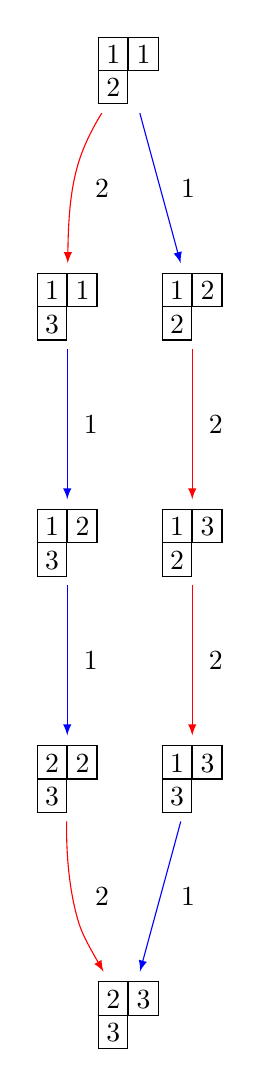
\begin{tikzpicture}[>=latex,line join=bevel,]
        %%
        \node (node_7) at (35.5bp,15.5bp) [draw,draw=none] {${\def\lr#1{\multicolumn{1}{|@{\hspace{.6ex}}c@{\hspace{.6ex}}|}{\raisebox{-.3ex}{$#1$}}}\raisebox{-.6ex}{$\begin{array}[b]{*{2}c}\cline{1-2}\lr{2}&\lr{3}\\\cline{1-2}\lr{3}\\\cline{1-1}\end{array}$}}$};
          \node (node_6) at (13.5bp,100.5bp) [draw,draw=none] {${\def\lr#1{\multicolumn{1}{|@{\hspace{.6ex}}c@{\hspace{.6ex}}|}{\raisebox{-.3ex}{$#1$}}}\raisebox{-.6ex}{$\begin{array}[b]{*{2}c}\cline{1-2}\lr{2}&\lr{2}\\\cline{1-2}\lr{3}\\\cline{1-1}\end{array}$}}$};
          \node (node_5) at (58.5bp,100.5bp) [draw,draw=none] {${\def\lr#1{\multicolumn{1}{|@{\hspace{.6ex}}c@{\hspace{.6ex}}|}{\raisebox{-.3ex}{$#1$}}}\raisebox{-.6ex}{$\begin{array}[b]{*{2}c}\cline{1-2}\lr{1}&\lr{3}\\\cline{1-2}\lr{3}\\\cline{1-1}\end{array}$}}$};
          \node (node_4) at (13.5bp,185.5bp) [draw,draw=none] {${\def\lr#1{\multicolumn{1}{|@{\hspace{.6ex}}c@{\hspace{.6ex}}|}{\raisebox{-.3ex}{$#1$}}}\raisebox{-.6ex}{$\begin{array}[b]{*{2}c}\cline{1-2}\lr{1}&\lr{2}\\\cline{1-2}\lr{3}\\\cline{1-1}\end{array}$}}$};
          \node (node_3) at (13.5bp,270.5bp) [draw,draw=none] {${\def\lr#1{\multicolumn{1}{|@{\hspace{.6ex}}c@{\hspace{.6ex}}|}{\raisebox{-.3ex}{$#1$}}}\raisebox{-.6ex}{$\begin{array}[b]{*{2}c}\cline{1-2}\lr{1}&\lr{1}\\\cline{1-2}\lr{3}\\\cline{1-1}\end{array}$}}$};
          \node (node_2) at (58.5bp,185.5bp) [draw,draw=none] {${\def\lr#1{\multicolumn{1}{|@{\hspace{.6ex}}c@{\hspace{.6ex}}|}{\raisebox{-.3ex}{$#1$}}}\raisebox{-.6ex}{$\begin{array}[b]{*{2}c}\cline{1-2}\lr{1}&\lr{3}\\\cline{1-2}\lr{2}\\\cline{1-1}\end{array}$}}$};
          \node (node_1) at (58.5bp,270.5bp) [draw,draw=none] {${\def\lr#1{\multicolumn{1}{|@{\hspace{.6ex}}c@{\hspace{.6ex}}|}{\raisebox{-.3ex}{$#1$}}}\raisebox{-.6ex}{$\begin{array}[b]{*{2}c}\cline{1-2}\lr{1}&\lr{2}\\\cline{1-2}\lr{2}\\\cline{1-1}\end{array}$}}$};
          \node (node_0) at (35.5bp,355.5bp) [draw,draw=none] {${\def\lr#1{\multicolumn{1}{|@{\hspace{.6ex}}c@{\hspace{.6ex}}|}{\raisebox{-.3ex}{$#1$}}}\raisebox{-.6ex}{$\begin{array}[b]{*{2}c}\cline{1-2}\lr{1}&\lr{1}\\\cline{1-2}\lr{2}\\\cline{1-1}\end{array}$}}$};
          \draw [red,->] (node_0) ..controls (22.513bp,334.49bp) and (19.359bp,328.18bp)  .. (17.5bp,322.0bp) .. controls (15.067bp,313.92bp) and (13.896bp,304.8bp)  .. (node_3);
          \definecolor{strokecol}{rgb}{0.0,0.0,0.0};
          \pgfsetstrokecolor{strokecol}
          \draw (26.0bp,313.0bp) node {$2$};
          \draw [blue,->] (node_5) ..controls (51.019bp,72.504bp) and (46.184bp,55.054bp)  .. (node_7);
          \draw (57.0bp,58.0bp) node {$1$};
          \draw [red,->] (node_6) ..controls (13.112bp,74.388bp) and (14.001bp,60.622bp)  .. (17.5bp,49.0bp) .. controls (18.401bp,46.008bp) and (19.605bp,42.985bp)  .. (node_7);
          \draw (26.0bp,58.0bp) node {$2$};
          \draw [blue,->] (node_4) ..controls (13.5bp,157.62bp) and (13.5bp,140.39bp)  .. (node_6);
          \draw (22.0bp,143.0bp) node {$1$};
          \draw [red,->] (node_1) ..controls (58.5bp,242.62bp) and (58.5bp,225.39bp)  .. (node_2);
          \draw (67.0bp,228.0bp) node {$2$};
          \draw [blue,->] (node_3) ..controls (13.5bp,242.62bp) and (13.5bp,225.39bp)  .. (node_4);
          \draw (22.0bp,228.0bp) node {$1$};
          \draw [blue,->] (node_0) ..controls (42.981bp,327.5bp) and (47.816bp,310.05bp)  .. (node_1);
          \draw (57.0bp,313.0bp) node {$1$};
          \draw [red,->] (node_2) ..controls (58.5bp,157.62bp) and (58.5bp,140.39bp)  .. (node_5);
          \draw (67.0bp,143.0bp) node {$2$};
        %
        \end{tikzpicture}
    % \end{bla}
\end{figure}

% Check this against direct computation
%     \[
%     \partial_x z = 0 \qquad (\partial_y + x \partial_z)z = x
%     \]
% Something's off as 
% \[
% \varepsilon_1(z) \tilde e_1 (z) =  \young(11,3) \qquad \varepsilon_2(z) \tilde e_2 (z) = 0 
% \]
% Looks like the conventions are off. Since the tableau $\young(11,3)$ is weight $\alpha_2$ while $x$ is weight $\alpha_1$.
%  \varepsilon_1(b) \tilde e_1 (b) + \sum_{\varepsilon_1(b') < \varepsilon_1(b) - 1} c(b') b'

% For another example, the element $b = xy-z$ (the only other element of weight $\alpha_1 + \alpha_2$) has tableau $\young(13,2)$ which has $\varepsilon_1 = 0$ and $\varepsilon_2 = 1$. 

% Let's again check
% \[
%     \partial_x (xy-z) = y \qquad (\partial_y + x \partial_z) (xy-z) = x - x = 0 
% \]
% This time 
% \[
%     \varepsilon_1(xy-z) \tilde e_1 (xy-z) = 0  \qquad \varepsilon_2(xy-z) \tilde e_2 (xy-z) = \young(12,2)
% \]
% and the latter has weight $\alpha_1$ whereas $y$ has weight $\alpha_2$. 

\end{example}

\subsection*{The spherical case}

\subsection*{On Shapovalov forms}
% From talking to Daniel Juteau

Let $V$ be a representation of $G$ and fix a highest weight vector $v\in V$. In our case the representation is (the ``highest weight zero Verma'' appearing as) $V = \CC[U]$ and the highest weight vector is (probably) the weight zero vector $1_U\in U$. 

\begin{question}
    Can we get from the highest weight vector to any other MV basis vector by applying $f_i$ (or $e_i$ depending on the convention)? I think yes. 
\end{question}

The Shapovalov form is a bilinear form on $V$ normalized such that 
\begin{equation}
    (1_U,1_U) = 1
\end{equation}
and respecting 
\begin{equation}
    (a v , b u) = (v,a^*b u) 
\end{equation}
for any $a, b\in \{e_i,f_i\}$ and $e_i^* = f_i$\dots? 

Perhaps the easier thing (that we were meant) to consider is a ``piece'' of this ``highest weight'' form: The form of the (spherical, finite dimensional) highest weight $V(\lambda)$ irrep with highest weight vector $v_\lambda = [\{L_\lambda\}]$. Normalizing 
\begin{equation}
    (v_\lambda,v_\lambda) = 1
\end{equation}

In any case we are asking for a matrix $A$ such that $x^T A y = (x,y)$ where $x,y\in V$ or $V_\lambda$ are identified with their vector representations in the MV basis. In the MV basis $A$ has $(i,j)$ entry $(b_i,b_j)$ i.e.\ $e_i^T A e_j = (b_i,b_j)$. So we'd have to figure out the path to $b_i, b_j$ from $1_U$ or $v_\lambda$ and apply it. 

\begin{question}
    How is this the equivalent of Mirkovi\'c's question? 
\end{question}

% \bibliography{abc}
% https://arxiv.org/pdf/1206.3647.pdf
% https://mathoverflow.net/questions/338315/shapovalov-form-on-verma-modules
% Total positivity, Schubert positivity, and Geometric Satake by Thomas Lam and Konstanze Reitsche